\documentclass{beamer}


\newcommand{\lesson}{Object-Oriented Programming, Part 2 of 3}
\newcommand{\shorttitle}{OOP2}



\newcommand{\course}{Introduction to Object-Oriented Programming}
\subject{\course}
\title[\lesson]{\course}
\subtitle{\lesson}

\author[CS 1331]
{Christopher Simpkins \\\texttt{chris.simpkins@gatech.edu}}
\institute[Georgia Tech]

\date[]{}

\newcommand{\link}[2]{\href{#1}{\textcolor{blue}{\underline{#2}}}}
\newcommand{\code}{http://www.cs1331.org/code}

\usepackage{colortbl}

% If you have a file called "university-logo-filename.xxx", where xxx
% is a graphic format that can be processed by latex or pdflatex,
% resp., then you can add a logo as follows:

% \pgfdeclareimage[width=0.6in]{coc-logo}{cc_2012_logo}
% \logo{\pgfuseimage{coc-logo}}

\mode<presentation>
{
  \usetheme{Berlin}
  \useoutertheme{infolines}

  % or ...

 \setbeamercovered{transparent}
  % or whatever (possibly just delete it)
}

\usepackage{tikz}
% Optional PGF libraries
\usepackage{pgflibraryarrows}
\usepackage{pgflibrarysnakes}
\usepackage{pgfplots}
\usepackage{fancybox}
\usepackage{listings}
\usepackage{hyperref}
\hypersetup{colorlinks=true,urlcolor=blue}
\usepackage[english]{babel}
% or whatever

\usepackage[latin1]{inputenc}
% or whatever

\usepackage{times}
\usepackage[T1]{fontenc}
% Or whatever. Note that the encoding and the font should match. If T1
% does not look nice, try deleting the line with the fontenc.


\usepackage{listings}

% "define" Scala
\lstdefinelanguage{scala}{
  morekeywords={abstract,case,catch,class,def,%
    do,else,extends,false,final,finally,%
    for,if,implicit,import,match,mixin,%
    new,null,object,override,package,%
    private,protected,requires,return,sealed,%
    super,this,throw,trait,true,try,%
    type,val,var,while,with,yield},
  otherkeywords={=>,<-,<\%,<:,>:,\#,@},
  sensitive=true,
  morecomment=[l]{//},
  morecomment=[n]{/*}{*/},
  morestring=[b]",
  morestring=[b]',
  morestring=[b]""",
}

\usepackage{color}
\definecolor{dkgreen}{rgb}{0,0.6,0}
\definecolor{gray}{rgb}{0.5,0.5,0.5}
\definecolor{mauve}{rgb}{0.58,0,0.82}

% Default settings for code listings
\lstset{frame=tb,
  language=scala,
  aboveskip=2mm,
  belowskip=2mm,
  showstringspaces=false,
  columns=flexible,
  basicstyle={\scriptsize\ttfamily},
  numbers=none,
  numberstyle=\tiny\color{gray},
  keywordstyle=\color{blue},
  commentstyle=\color{dkgreen},
  stringstyle=\color{mauve},
  frame=single,
  breaklines=true,
  breakatwhitespace=true,
  keepspaces=true
  %tabsize=3
}


% \beamerdefaultoverlayspecification{<+->}


\begin{document}

\begin{frame}
  \titlepage
\end{frame}

%------------------------------------------------------------------------
\begin{frame}[fragile]{Fitting Classes Into the Java Hierarchy}


{\tt java.lang.Object} defines several methods that are designed to be overriden in subclasses (\href{http://docs.oracle.com/javase/specs/jls/se7/html/jls-4.html#jls-4.3.2}{JLS \S 4.3.2}:)
\begin{itemize}
\item The method {\tt equals(Object)} defines a notion of object equality, which is based on value, not reference, comparison.
\item The method {\tt hashCode} is very used together with  {\tt equals(Object)} in hashtables such as {\tt java.util.Hashmap}.
\item The method {\tt toString} returns a {\tt String} representation of the object.
\item The method {\tt clone} is used to make a duplicate of an object (don't touch).
\item The method {\tt finalize} is run just before an object is destroyed (don't touch).
\end{itemize}

A class hierarchy is also sometimes called a {\it framework}.

\end{frame}
%------------------------------------------------------------------------


%------------------------------------------------------------------------
\begin{frame}[fragile]{When to Override the {\tt equals(Object)} Method}


The default implementation of {\tt equals(Object)} in {\tt java.lang.Object} is object identity - each object {\tt equals(Object)} only itself.

When should a class override {\tt equals(Object)}?
\begin{itemize}
\item When logical equality differs from object identity, as is the case for {\it value} classes like {\tt Date}
\item When classes don't implement instance control.
  \begin{itemize}
  \item Instance control means that a class ensures that there is only one instance of a class.
  \end{itemize}
\item When a suitable {\tt equals(Object)} method is not provided by a superclass.
\end{itemize}

More important than recognizing {\it when} to override {\tt equals(Object)} is knowing {\it how} to override {\tt equals(Object)}.
\end{frame}
%------------------------------------------------------------------------

%------------------------------------------------------------------------
\begin{frame}[fragile]{How to Override the {\tt equals(Object)} Method}


Obey the general contract of {\tt equals(Object)} (\href{}{JLS }), which says that {\tt equals(Object)} defines an equivalence relation.  So, for non-null references, {\tt equals(Object)} is
\begin{itemize}
\item reflexive - any object {\tt equals(Object)} itself
\item symmetric - if {\tt a.equals(Object)(b)} is true then {\tt b.equals(a)} must be true
\item transitive - if {\tt a.equals(b)} and {\tt b.equals(c)} are true then {\tt a.equals(c)} must be true
\item consistent - if {\tt a} and {\tt b} do not change between invocations of {\tt a.equals(b)} or {\tt b.equals(a)} then each invocation must return the same result
\item {\tt a.equals(null)} must always return {\tt false}.
\end{itemize}


\end{frame}
%------------------------------------------------------------------------


%------------------------------------------------------------------------
\begin{frame}[fragile]{A Recipe for Implementing {\tt equals(Object)}}


Obeying the general contract of {\tt equals(Object)} is easier if you follow these steps.\\

\begin{enumerate}
\item Ensure the other object is not null.
\item Check for reference equality with == (are we comparing to self?).
\item Check that the other object is an {\tt instanceof} this object's class.
\item Cast the other object to this's type (guaranteed to work after instanceof test)
\item Check that each ``significant'' field in the other object {\tt equals(Object)} the corresponding field in this object.
\end{enumerate}

After seeing an example applicaiton of this recipe we'll motivate the proper implementation of {\tt equals(Object)} methods by introducing our first collection class, {\tt ArrayList}.

\end{frame}
%------------------------------------------------------------------------

%------------------------------------------------------------------------
\begin{frame}[fragile]{An Example {\tt equals(Object)} Method}

Assume we have a {\tt Person} class with a single {\tt name} field.
\begin{enumerate}
\item Ensure the other object is not null.
\item Check for reference equality with == (are we comparing to self?).
\item Check that the other object is an {\tt instanceof} this object's class.
\item Cast the other object to this's type (guaranteed to work after instanceof test)
\item Check that each ``significant'' field in the other object {\tt equals(Object)} the corresponding field in this object.
\end{enumerate}
Applying the recipe:
\begin{lstlisting}[language=Java]
        public boolean equals(Object other) {
1:          if (null == other) { return false; }
2:          if (this == other) { return true; }
3:          if (!(other instanceof Person)) { return false; }
4:          Person that = (Person) other;
5:          return this.name.equals(that.name);
        }
\end{lstlisting}

\end{frame}
%------------------------------------------------------------------------

%------------------------------------------------------------------------
\begin{frame}[fragile]{Arrays and {\tt ArrayList}}


\begin{itemize}
\item Arrays are fixed-size collections of any data types, including primitives
\item {\tt ArrayList}s are dynamically-allocated (i.e., automatically resized) collections of reference types (not primitives - but we'll talk about autoboxing).
\item {\tt ArrayList}s use arrays internally, but this isn't important to know for basic use.
\end{itemize}


\end{frame}
%------------------------------------------------------------------------

%------------------------------------------------------------------------
\begin{frame}[fragile]{{\tt ArrayList} Basics}


Create an {\tt ArrayList} with operator {\tt new}:
\begin{lstlisting}[language=Java]
  ArrayList tasks = new ArrayList();
\end{lstlisting}
Add items with {\tt add()}:
\begin{lstlisting}[language=Java]
  tasks.add("Eat");
  tasks.add("Sleep");
  tasks.add("Code");
\end{lstlisting}
Traverse with for-each loop:
\begin{lstlisting}[language=Java]
  for (Object task: tasks) {
      System.out.println(task);
  }
\end{lstlisting}

Note that the for-each loop implicitly uses an iterator.

\end{frame}
%------------------------------------------------------------------------
%------------------------------------------------------------------------
\begin{frame}[fragile]{Primitives in Collections}

{\tt ArrayList}s can only hold reference types.  So you must use wrapper classes for primitives:
\begin{lstlisting}[language=Java]
  ArrayList ints = new ArrayList();
  ints.add(new Integer(42));
\end{lstlisting}
Java auto-boxes primitives when adding to a collection:
\begin{lstlisting}[language=Java]
  ints.add(99);
\end{lstlisting}
But auto-unboxing can't be done when retrieving from an untyped collection:
\begin{lstlisting}[language=Java]
  int num = ints.get(0); // won't compile
\end{lstlisting}
The old way to handle this with untyped collections is to cast it:
\begin{lstlisting}[language=Java]
int num = (Integer) ints.get(0); // auto-unboxing on assignment to int
\end{lstlisting}
We'll see a better way to handle this with generics.

See \link{\code/collections/ArrayListPrimitivesDemo.java}{ArrayListPrimitivesDemo.java} for more.
\end{frame}
%------------------------------------------------------------------------

%------------------------------------------------------------------------
\begin{frame}[fragile]{The {\tt equals(Object)} Method and Collections}



\begin{itemize}
\item A class whose instances will be stored in a collection must have a properly implemented {\tt equals(Object)} method.
\item The {\tt contains} method in collections uses the {\tt equals(Object)} method in the stored objects.
\item The default implementation of {\tt equals(Object)} (object identity - true only for same object in memory) only rarely gives correct results.
\item Note that {\tt hashcode()} also has a defualt implementation that uses the object's memory address.  As a rule, whenever you override {\tt equals(Object)}, you should also override {\tt hashcode}\footnote{{\tt hashcode()} is used in objects that are keys in {\tt Map}s.  You'll learn about {\tt Map}s later in the course.}.
\end{itemize}


\end{frame}
%------------------------------------------------------------------------

%------------------------------------------------------------------------
\begin{frame}[fragile]{{\tt equals(Object)} Method Examples}

\vspace{-.05in}
In this simple class hierarchy, {\tt FoundPerson} has a properly implemented {\tt equals(Object)} method and {\tt LostPerson} does not.
\vspace{-.05in}
\begin{lstlisting}[language=Java]
    abstract static class Person {
        public String name;
        public Person(String name) {
            this.name = name;
        }
    }
    static class LostPerson extends Person {
        public LostPerson(String name) { super(name); }
    }
    static class FoundPerson extends Person {
        public FoundPerson(String name) { super(name); }

        public boolean equals(Object other) {
            if (this == other) { return true; }
            if (!(other instanceof Person)) { return false; }
            return ((Person) other).name.equals(this.name);
        }
    }
\end{lstlisting}
\vspace{-.05in}
Let's examine the code in \link{\code/collections/ArrayListEqualsDemo.java}{ArrayListEqualsDemo.java}.

\end{frame}
%------------------------------------------------------------------------

%------------------------------------------------------------------------
\begin{frame}[fragile]{Override-Equivalence}

Two methods are \href{http://docs.oracle.com/javase/specs/jls/se8/html/jls-8.html#jls-8.4.2}{override-equivalent} if:
\begin{itemize}
\item they have the same name,
\item they have the same parameter lists, and
\item their return values are \link{http://docs.oracle.com/javase/tutorial/java/javaOO/returnvalue.html}{covariant}
\end{itemize}

These rules lead to a few pitfalls:

\begin{itemize}
\item You can't define override-equivalent methods in the same class.
\item In subclasses it's easy to accidentally overload a superclass method when you meant to override.
\end{itemize}

Let's look at a few examples to help us understand these rules.

\end{frame}
%------------------------------------------------------------------------

%------------------------------------------------------------------------
\begin{frame}[fragile]{Covariant Returns}
\vspace{-.05in}
{\tt covariantReturn} is covariant in {\tt Person} and {\tt LostPerson}:
\vspace{-.05in}
\begin{lstlisting}[language=Java]
abstract static class Person {
    public String name;
    public Person(String name) { this.name = name; }
    public Object covariantReturn() { return new Object(); }
}
static class LostPerson extends Person {
    public LostPerson(String name) { super(name); }
    @Override public LostPerson covariantReturn() { return this; }
}
\end{lstlisting}
... because {\tt LostPerson} is a subtype of {\tt Object}.\\
But {\tt SubLostPerson} won't compile:
\vspace{-.05in}
\begin{lstlisting}[language=Java]
static class SubLostPerson extends LostPerson {
    public SubLostPerson(String name) { super(name); }
    @Override public Person covariantReturn() { return this; }
}
\end{lstlisting}
... becuase its {\tt covariantReturn}'s return type is {\it contravariant}, that is, {\tt Person} is a supertype of {\tt LostPerson}.
\end{frame}
%------------------------------------------------------------------------


%------------------------------------------------------------------------
\begin{frame}[fragile]{Non-Covariant Return}

{\tt NoncompilingPerson} won't compile because {\tt int} is not a subtype of {\tt boolean} and because return-type covariance only applies to reference types, not primitives.
\begin{lstlisting}[language=Java]
    static class NonCompilingPerson extends Person {
        public NonCompilingPerson(String name) { super(name); }

        /**
         * This method won't compile because int is not a subtype of boolean.
         */
        public int equals(Object other) {
            if (null == other) return 0;
            if (this == other) return 1;
            if (!(other instanceof Person)) return 0;
            return ((Person) other).name.equals(this.name) ? 1 : 0;
        }
    }

\end{lstlisting}


\end{frame}
%------------------------------------------------------------------------

%------------------------------------------------------------------------
\begin{frame}[fragile]{Accidental Overloading}

It's easy to make this mistake:
\begin{lstlisting}[language=Java]
    static class OverloadedPerson extends Person {
        public OverloadedPerson(String name) { super(name); }

        public boolean equals(OverloadedPerson other) {
            if (null == other) { return false; }
            if (this == other) { return true; }
            if (!(other instanceof OverloadedPerson)) { return false; }
            return ((OverloadedPerson) other).name.equals(this.name);
        }
    }
\end{lstlisting}

\begin{itemize}
\item Signature of {\tt equals} in {\tt Object} is {\tt public boolean equals(Object other)} - parameter type is {\tt Object}.
\item In {\tt OverloadedPerson} we've accidentally {\it overloaded} {\tt equals} instead of {\it overriding} {\tt equals} by making the parameter type {\tt OverloadedPerson}.
\end{itemize}

Using the {\tt @Override} annotation helps you avoid this mistake.

\end{frame}
%------------------------------------------------------------------------

%------------------------------------------------------------------------
\begin{frame}[fragile]{Closing Thoughts}

\begin{itemize}
\item {\tt java.lang.Object} is the root superclass of every Java class.
\item "Classic" Java collections are general because they hold elements of type {\tt Object}
\item Java collections and many programming idioms rely on the methods defined in {\tt Object}, some of which must be overridden in subclasses in order for instances of these subclasses to function properly as elements of collections.
\item Overriding {\tt equals} is straightforward if you follow the recipe.
\item There's more to overriding {\tt equals} -- in particular, overriding {\tt hashcode} -- but now we know the basic concepts.
\end{itemize}

\end{frame}
%------------------------------------------------------------------------



%% %------------------------------------------------------------------------
%% \begin{frame}[fragile]{SummerIntern}


%% Let's add a summer intern class to our Employee hierarchy.
%% \begin{lstlisting}[language=Java]
%% public class SummerIntern extends HourlyEmployee {

%%     public SummerIntern(String name, Date hireDate) {
%%         this(name, hireDate, 20.00, 160.0);
%%     }
%%     public SummerIntern(String name, Date hireDate,
%%                         double hourlyWage, double monthlyHours) {
%%         super(name, hireDate, hourlyWage, monthlyHours);
%%     }
%%     public double monthlyPay() {
%%         Calendar rightNow = Calendar.getInstance();
%%         return isSummer(rightNow) ? super.monthlyPay() : 0.0;
%%     }
%%     // ...
%% }
%% \end{lstlisting}

%% Will this compile?

%% \end{frame}
%% %------------------------------------------------------------------------


%% %------------------------------------------------------------------------
%% \begin{frame}[fragile]{The {\tt Employee} Class Hierarchy}


%% Now we have an expanded {\tt Employee} class hierarchy:
%% \vspace{-.1in}
%% \begin{center}
%% 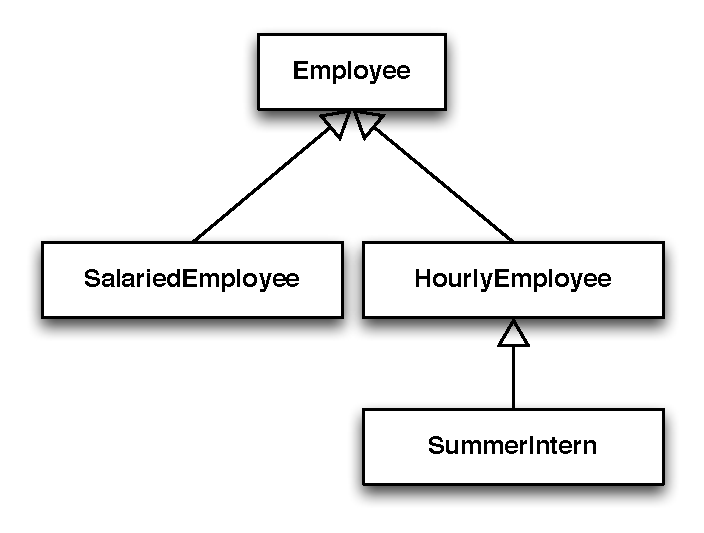
\includegraphics[height=1.5in]{expanded-employee-class-hierarchy.pdf}
%% \end{center}

%% \begin{itemize}
%% \item We can get the payRoll for the current month by making use of the polymorphic {\tt getMonthlyPay} method.
%% \item What if we wanted to get the payroll for a particular month?
%% \end{itemize}

%% Let's overload {\tt monthlyPay} so we can get the payroll for any month, not just the current month.

%% \end{frame}
%% %------------------------------------------------------------------------


%% %------------------------------------------------------------------------
%% \begin{frame}[fragile]{Overloading Methods}


%% An overloaded method is a set of methods with the same names but different signatures (different return types and/or parameter lists)\footnote{More precisely, two methods with the same name whose signatures are not {\it override-equivalent} are overloaded.} (\href{http://docs.oracle.com/javase/specs/jls/se7/html/jls-8.html#jls-8.4.9}{JLS \S 8.4.9}).\\
%% \vspace{.1in}
%% Here's an overloaded {\tt monthlyPay}
%% \begin{lstlisting}[language=Java]
%% public double monthlyPay() {
%%     Calendar rightNow = Calendar.getInstance();
%%     return monthlyPay(rightNow);
%% }

%% public double monthlyPay(Calendar calendar) {
%%     return isSummer(calendar) ? super.monthlyPay() : 0.0;
%% }
%% \end{lstlisting}

%% \begin{itemize}
%% \item In which classes should these methods be defined?
%% \end{itemize}


%% \end{frame}
%% %------------------------------------------------------------------------

%% %------------------------------------------------------------------------
%% \begin{frame}[fragile]{The {\tt Employee} Class Hierarchy in UML}


%% \vspace{-.2in}
%% \begin{center}
%% 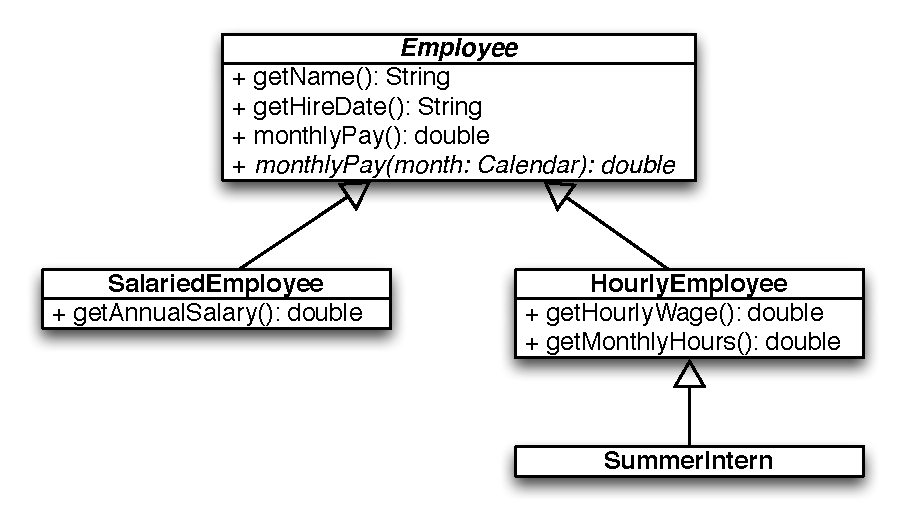
\includegraphics[height=1.5in]{employee-uml.pdf}
%% \end{center}
%% \vspace{-.25in}
%% \begin{itemize}
%% \item Italicized names are abstract (e.g., {\it Employee} is an abstract class, {\it + getMonthlyPay(month: Calendar)} is an abstract method).
%% \item We've only shown public methods (denoted by the '+' symbols in front of their names).
%% \item Each class has all the public methods in its superclasses, and possibly additional methods.
%% \item {\tt SummerIntern} only {\it specializes} {\tt HourlyEmployee}, that is, it modifies some behavior of its superclass but does not add any additional behavior.
%% \end{itemize}


%% \end{frame}
%% %------------------------------------------------------------------------

%% %------------------------------------------------------------------------
%% \begin{frame}[fragile]{Forecasting Payroll}


%% Now with our overloaded  {\tt montlyPay} method we can forecast payroll:
%% \begin{lstlisting}[language=Java]
%% Company c = new Company("employees.data");
%% Calendar may =  Calendar.getInstance();
%% may.set(Calendar.MONTH, Calendar.MAY);
%% Calendar june = Calendar.getInstance();
%% june.set(Calendar.MONTH, Calendar.JUNE);
%% System.out.println(c.employees.get(0).monthlyPay());
%% System.out.printf("Monthly payroll for May: %.2f%n",
%%                   c.monthlyPayroll(may));
%% System.out.printf("Monthly payroll for June: %.2f%n",
%%                   c.monthlyPayroll(june));
%% \end{lstlisting}

%% Let's play with these classes.


%% \end{frame}
%% %------------------------------------------------------------------------



% %------------------------------------------------------------------------
% \begin{frame}[fragile]{}


% \begin{lstlisting}[language=Java]

% \end{lstlisting}

% \begin{itemize}
% \item
% \end{itemize}


% \end{frame}
% %------------------------------------------------------------------------


\end{document}
